%----------------------------------------------------------------------------------------
%	Capítulo 4
%----------------------------------------------------------------------------------------

\pagestyle{myportland}
\pagenumbering{arabic}
\doublespacing
\chapter[\quad\quad\quad\quad ----- Antecedentes]{\\Antecedentes}
\thispagestyle{myportland}

En este capítulo se explica la procedencia del diseño junto con su propósito en la descripción del sistema conceptual. Luego, se explaya el objetivo general y los objetivos específicos del presente trabajo, el alcance del estudio y la metodología usada.


\begin{myfigure}[H]
	\centering
	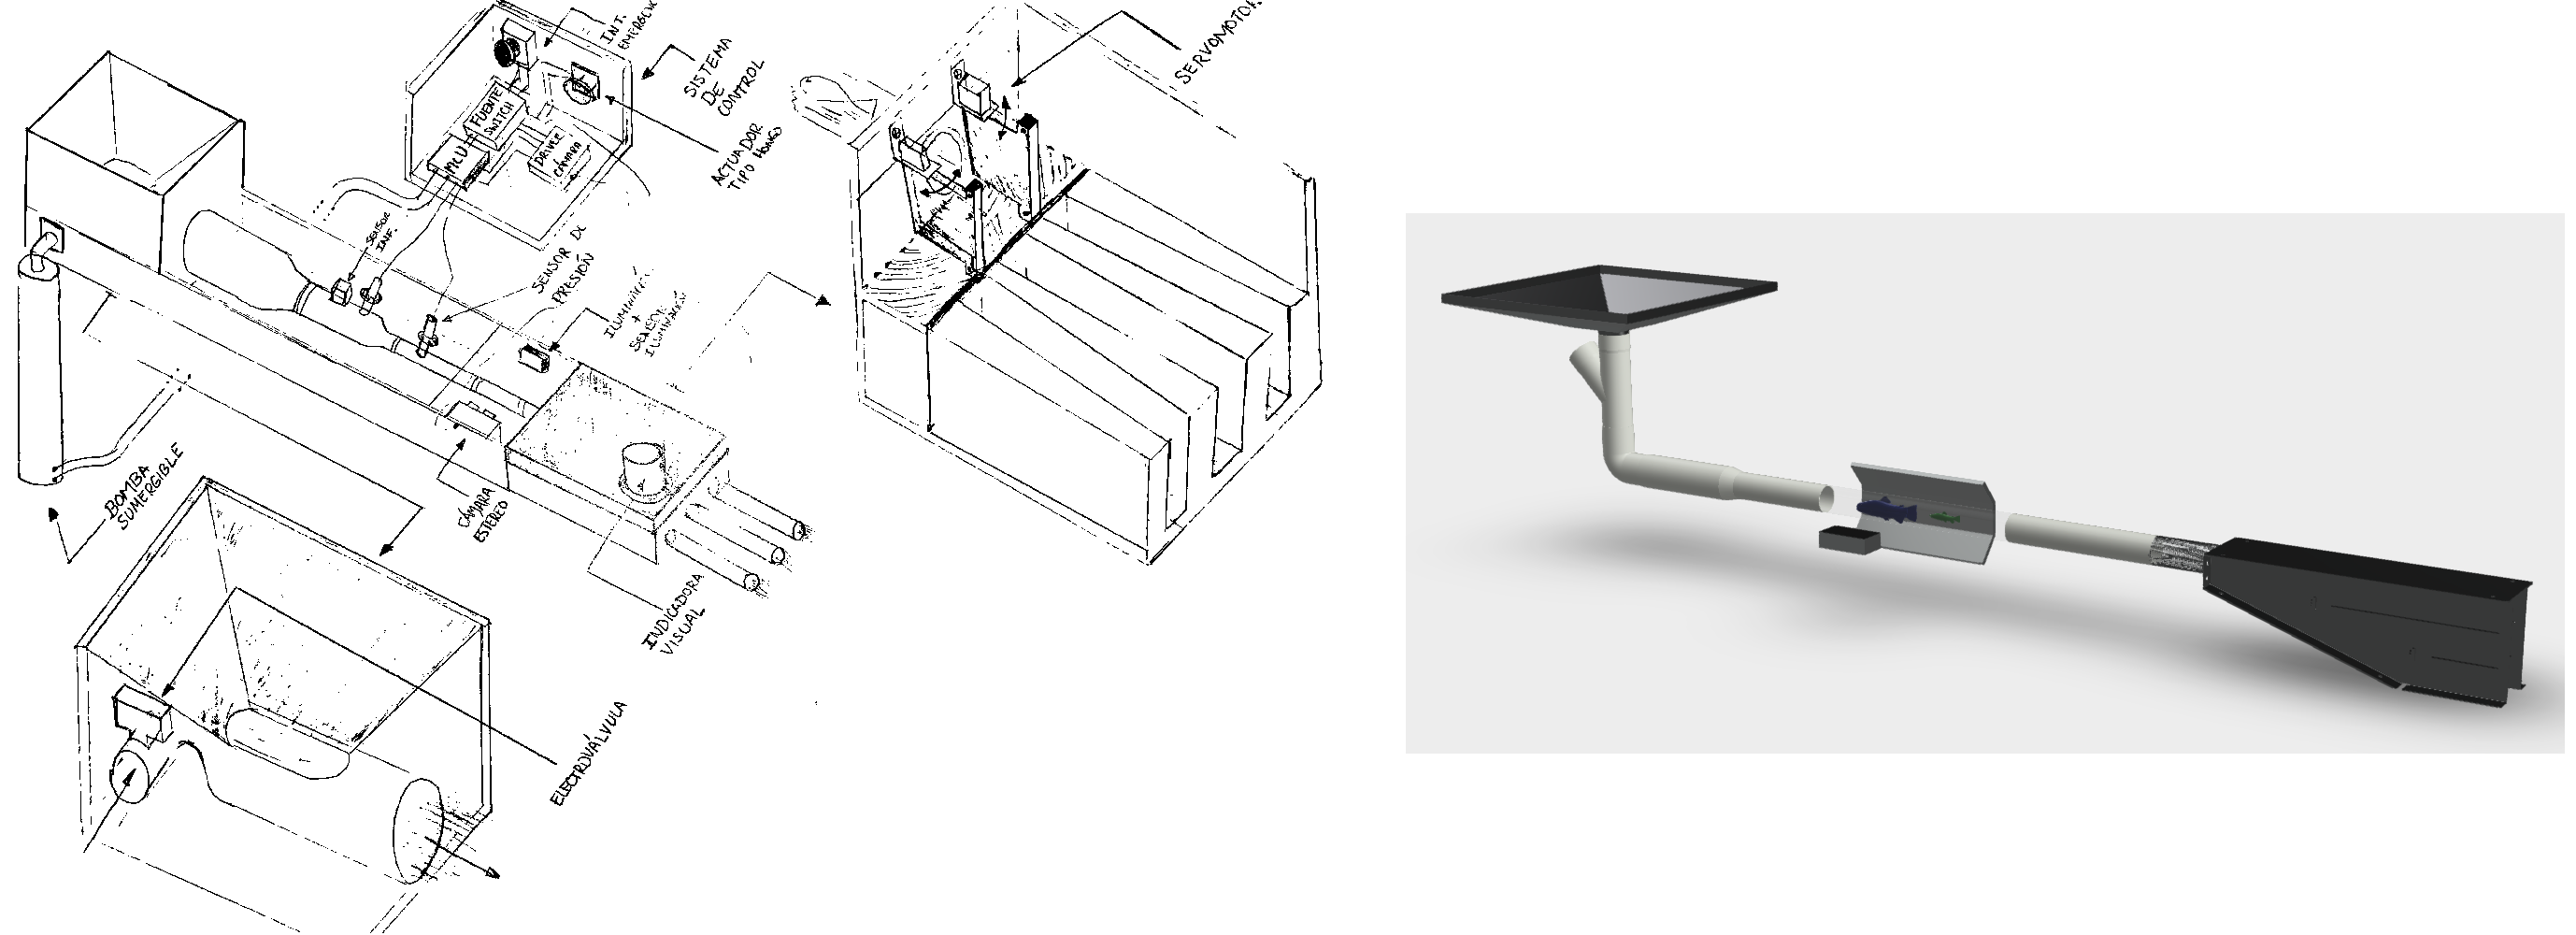
\includegraphics[width=1\textwidth]{chapter4/concepto optimo dibujo y virtual.png}
	\caption{Dibujo del concepto óptimo}
	\begin{myflushcenter}
		Fuente: \cite{DiazVergara2020}.
	\end{myflushcenter}
	\label{fig:concepto optimo dibujo y virtual}
\end{myfigure}

\vspace{-2.0em}

%% NUEVA SECCIÓN X.X
\section{Problemática}
%\label{sec:descripcion del sistema conceptual}

El presente trabajo es la continuación del trabajo \textit{"Diseño conceptual de clasificadora y contadora de truchas arcoíris (Oncorhynchus mykiss) de 10 a 20 centímetros para la crianza de truchas en la Laguna de Paucarcocha"}\footnote{\cite{DiazVergara2020}}: parte del diseño conceptual y, en el presente trabajo, se desarrolla el diseño integral. Dicho diseño conceptual se enfoca en elaborar un sistema que "reduzca la mortandad presente en el proceso de clasificación manual". En la Figura \ref{fig:concepto optimo dibujo y virtual} se muestra el bosquejo del concepto de solución desarrollado en dicho trabajo y también una versión 3D sobre dicho bosquejo sin algunos componentes. El presente trabajo continua en brindar una solución de ingeniería que logre disminuir las consecuencias de un trabajo manual con maquinaria semi-automática.


%% NUEVA SECCIÓN X.X
\section{Alcance}

El presente estudio abarca el diseño integral de la máquina clasificadora y contadora de truchas arcoíris (CCT) con enfoque en el costo para disminuir la mortalidad en el proceso de clasificación y conteo de truchas en lagos o lagunas. Asimismo, unifica tecnologías de la última generación para automatizar el proceso mencionado. El diseño integral abarca el diseño de la máquina centrado en los operarios, el uso de tecnologías recientes para brindar un sistema que unifica acceso mediante aplicaciones, procesamiento offline e interacción mediante aplicaciones móviles. Además, este diseño pretende ser la base de un prototipo y posterior máquina comercializable para mejorar la producción de salmones en lagos y lagunas en el Perú. Este sistema esta dentro de los objetivos globales de desarrollo sostenible establecidos por la ONU\footnote{Las Naciones Unida. Ver objetivos en \href{https://www.un.org/sustainabledevelopment/es/objetivos-de-desarrollo-sostenible/}{https://www.un.org/sustainabledevelopment/es/objetivos-de-desarrollo-sostenible/}}: noveno objetivo que trata sobre industria, innovación e infraestructura, en este caso en el sector acuícola.

%% NUEVO SUBSECCION X.X
\section{Objetivos}

Se presenta el objetivo general y los objetivos específicos del presente trabajo.

%% NUEVA SUB-SUB-SECCION X.X.X
\subsection{Objetivo general}

Realizar el diseño integral (de ingeniería) de una máquina clasificadora y contadora de truchas arcoíris (CCT) de 15 a 20 centímetros a partir del diseño conceptual previo\footnote{Diseño conceptual extraído de \cite{DiazVergara2020}}.

%% NUEVA SUB-SUB-SECCION X.X.X
\subsection{Objetivos específicos}

\begin{itemize}
	\item Diseñar la máquina de clasificación y conteo de truchas, un sistema de procesamiento de imágenes y un sistema que permita su control e interacción con los operarios.
	\item Recolectar y etiquetar imágenes para formar una base de datos para el algoritmo de detección de truchas en el sistema de procesamiento de imágenes.
	\item Realizar pruebas conceptuales de los algoritmos, análisis de falla mecánica y presentar resultados de los algoritmos seleccionados.
	\item Presentar una estimación de costos del diseño, componentes, materiales y manufactura.
	%%%%%%%%%%%%%%%%%%%%%%%%%%%%%%%%%%%%%%%%%%%%%%%%%%%%%%%%%%%%%%%%%%%%%%%%%%%%%%%%%%%%%%%
	%\textcolor{blue}{[BORRADOR] ¿Alcanzará el tiempo o uso una red neuronal pre-entrenada? [/BORRADOR]} 
	%%%%%%%%%%%%%%%%%%%%%%%%%%%%%%%%%%%%%%%%%%%%%%%%%%%%%%%%%%%%%%%%%%%%%%%%%%%%%%%%%%%%%%%
	%\item Desarrollar el sistema de procesamiento de imágenes para la detección y conteo de truchas arcoíris.
	%\item Orientar el desarrollo del proyecto hacia una máquina de bajo costo y con durabilidad.
\end{itemize}



%% NUEVO SUBSECCION X.X
\section{Metodología}

En la sección llamada \textit{"Desarrollo del diseño mecatrónico conceptual"} \footnote{\cite{DiazVergara2020}} se analizó el concepto de solución óptimo. En la Figura \ref{fig:estado diseno mecatronico etapa 3} se muestra la etapa final de unir las sub-soluciones para desarrollar una forma viable de implementarlos de una forma integral.

\begin{myfigure}[H]
	\footnotesize\centering
	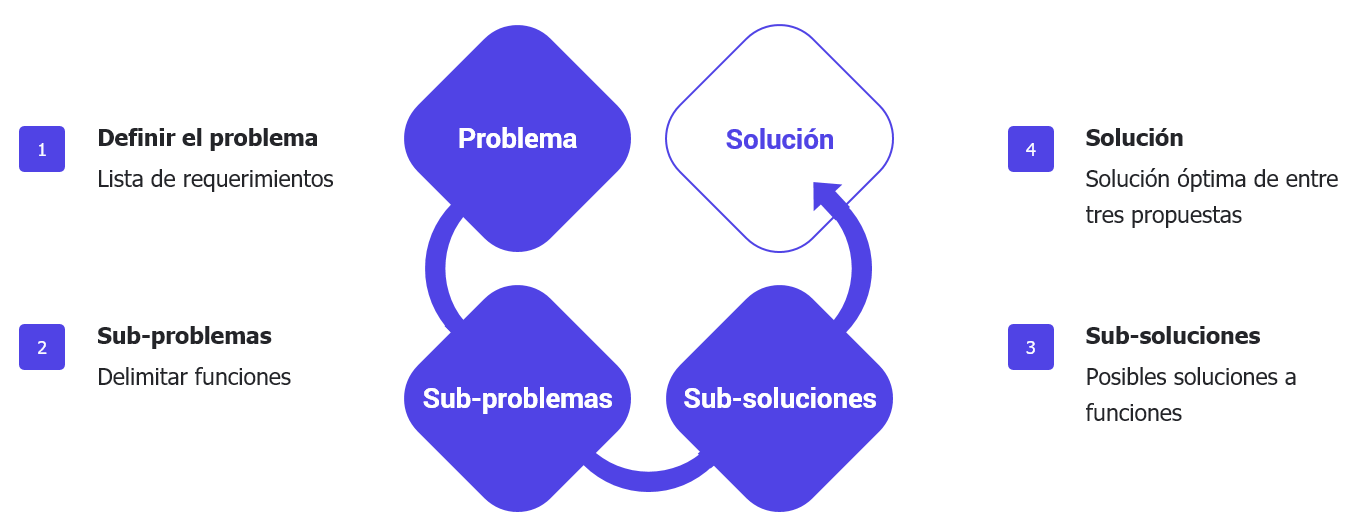
\includegraphics[width=1\textwidth]{chapter5/estado diseno subsoluciones.png}
	\caption{Estado de diseño mecatrónico: sub-soluciones}
	\begin{myflushcenter}
		Fuente: Elaboración propia
	\end{myflushcenter}
	\label{fig:estado diseno mecatronico etapa 3}
\end{myfigure}

Según el proceso de diseño indicado en la norma VDI 2221 que se muestra en la Figura \ref{fig:vdi2221} se parte del diseño conceptual propuesto (5) y se presenta el diseño integral (6)\footnote{\cite{Pahl2007}}, también llamado diseño de ingeniería, que abarca diferentes puntos: dimensionamiento del sistema; cálculos; selección técnica de materiales entorno a su aplicación; selección técnica de sensores; actuadores y dispositivos de control; lógica del control del sistema y su estrategia; planos mecánicos: ensamble y despiece; planos eléctricos y/o electrónicos; simulaciones de la máquina y una estimación de costos.

\begin{myfigure}[H]
	\footnotesize\centering
	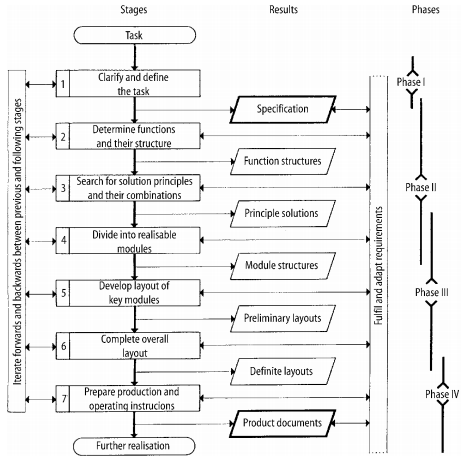
\includegraphics[width=0.75\textwidth]{chapter5/vdi2221.png}
	\caption{Fases de diseño según VDI 2221}
	\begin{myflushcenter}
		Fuente: \cite{Pahl2007}
	\end{myflushcenter}
	\label{fig:vdi2221}
\end{myfigure}

La metodología se refiere a los procesos que se emplean en el trabajo con el fin de cumplir los objetivos y presentar conclusiones. Debido a que los procedimientos son establecidos en las normas VDI 2221-2226, en las siguientes líneas se detalla los softwares utilizados para lograr el resultado brindado para el sistema en su conjunto. El desarrollo de ingeniería del concepto se realiza en el programa Fusion 360\footnote{\href{https://www.autodesk.com/products/fusion-360/overview}{Fusion360: "Integrated CAD, CAM, CAE, and PCB software"}}. Tanto los diseños como renders\footnote{Imágenes procesadas de un diseño para ser foto-realistas.} pueden ser visualizados online en la web mediante el uso de enlaces que son publicados en las secciones respectivas. Para el diseño electrónico se utiliza la página web EasyEDA\footnote{\href{https://easyeda.com/}{EasyEDA: An Easier and Powerful Online PCB Design Tool}.} debido a que cuenta con una extensa librería de componentes electrónicos y la fabricación de las PCBs en serie se realiza con pocos pasos y a un costo razonable. En cuánto al sistema de procesamiento de imágenes y sus instrucciones de procesamiento: como se acostumbra con sistema complejos se almacenan en Github\footnote{\href{https://github.com/}{Github: Development platform to review code, manage projects, and build software}.}; se desarrollan con librerías conocidas como PyTorch\footnote{\href{https://pytorch.org/}{PyTorch: An open source machine learning framework that accelerates the path from research prototyping to production deployment}.} apoyado de herramientas como Docker\footnote{\href{https://www.docker.com/}{Docker: Build and ship apps}.}, Heroku\footnote{\href{https://www.heroku.com/}{Heroku: Deploy, manage, and scale apps.}.}; en el caso del diseño frontend de la aplicación se realiza en la plataforma Figma\footnote{\href{https://www.figma.com/}{Figma: Create, test, and ship better designs from start to finish}.}. En cuanto al presente documento se realiza con \LaTeX y en el caso de los diagramas LucidChart\footnote{\href{https://www.lucidchart.com/}{LucidChart: Diagramación inteligente}.}.




